% AIPR 2026 poster, 48 x 36 in landscape. Build from this directory:
%   python -m src.analysis.poster_figures --evidence-root <tree> --output-dir docs/poster/generated
%   tectonic -X compile poster.tex
% Every number comes from generated/poster_macros.tex; none is typed here.
\documentclass[25pt,a0paper,margin=0mm,innermargin=22mm,colspace=18mm,
  subcolspace=0mm,blockverticalspace=16mm]{tikzposter}
\geometry{paperwidth=48in,paperheight=36in}
% tikzposter sized its canvas for A0 portrait at class load; re-derive it.
\makeatletter
\setlength{\TP@visibletextwidth}{\textwidth-2\TP@innermargin}
\setlength{\TP@visibletextheight}{\textheight-2\TP@innermargin}
\makeatother

\usepackage[T1]{fontenc}
\usepackage[sfdefault]{roboto}
\usepackage{amsmath,amssymb,booktabs,graphicx,qrcode,enumitem,array,ragged2e}
\usetikzlibrary{calc,positioning,arrows.meta,fit,backgrounds}
\graphicspath{{generated/}{../class_report/figures/static/}}
% GENERATED by src.analysis.poster_figures -- do not edit.
\def\PNBestCell{cnnin1k-f100-s0}
\def\PNBestCellFinal{0.574}
\def\PNBestCellTest{0.888}
\def\PNCells{32}
\def\PNCnnOpticalFinalGainMin{+0.038}
\def\PNCnnOpticalTestGainMax{+0.063}
\def\PNCnnOpticalTestGainMin{+0.025}
\def\PNCnnSarTestDropFiftySixOneEleven{0.026}
\def\PNCodeSha{06b2e61}
\def\PNFinalCnnBestTwelve{0.501}
\def\PNFinalCnnBestTwelveRole{SAR}
\def\PNFinalCnnRandomOneEleven{0.511}
\def\PNFinalCnnSarMinusOptTen{+0.045}
\def\PNFinalCnnSarMinusOptHundred{$-$0.073}
\def\PNFinalCnnSarMinusOptTwentyFive{+0.014}
\def\PNFinalCnnSarMinusOptFifty{$-$0.006}
\def\PNFinalDark{3{,}644}
\def\PNFinalDarkRecallMax{0.228}
\def\PNFinalDarkRecallMin{0.136}
\def\PNFinalFOneMax{0.574}
\def\PNFinalFOneMin{0.409}
\def\PNFinalGainTwelveMax{+0.111}
\def\PNFinalGainTwelveMin{+0.048}
\def\PNFinalNearShore{2{,}686}
\def\PNFinalNearShoreFOneMax{0.041}
\def\PNFinalNearShoreFOneMin{0.015}
\def\PNFinalPrecisionMax{0.909}
\def\PNFinalPrecisionMin{0.639}
\def\PNFinalRecallMax{0.434}
\def\PNFinalRecallMin{0.286}
\def\PNFinalScenes{50}
\def\PNFinalVessels{8{,}642}
\def\PNFinalVitBestTwelve{0.523}
\def\PNFinalVitBestTwelveRole{ImageNet}
\def\PNFinalVitRandomOneEleven{0.522}
\def\PNFinalVitSarMinusOptTen{+0.008}
\def\PNFinalVitSarMinusOptHundred{$-$0.003}
\def\PNFinalVitSarMinusOptTwentyFive{$-$0.081}
\def\PNFinalVitSarMinusOptFifty{+0.053}
\def\PNGpuHours{567.6}
\def\PNMeanTestMinusFinal{0.306}
\def\PNRerunCells{28}
\def\PNRerunMax{0.043}
\def\PNRerunMean{0.008}
\def\PNStemDevAfter{0.837}
\def\PNStemDevBefore{0.799}
\def\PNStemWeightNormRatio{5.85$\times$}
\def\PNTestCnnBestTwelve{0.800}
\def\PNTestCnnBestTwelveRole{SAR}
\def\PNTestCnnRandomOneEleven{0.816}
\def\PNTestCnnSarMinusOptTen{+0.080}
\def\PNTestCnnSarMinusOptHundred{$-$0.018}
\def\PNTestCnnSarMinusOptTwentyFive{+0.052}
\def\PNTestCnnSarMinusOptFifty{+0.026}
\def\PNTestFOneMax{0.888}
\def\PNTestFOneMin{0.657}
\def\PNTestGainTwelveMax{+0.143}
\def\PNTestGainTwelveMin{+0.063}
\def\PNTestScenes{16}
\def\PNTestVitBestTwelve{0.813}
\def\PNTestVitBestTwelveRole{ImageNet}
\def\PNTestVitRandomOneEleven{0.831}
\def\PNTestVitSarMinusOptTen{$-$0.002}
\def\PNTestVitSarMinusOptHundred{+0.029}
\def\PNTestVitSarMinusOptTwentyFive{$-$0.066}
\def\PNTestVitSarMinusOptFifty{+0.028}
\def\PNVitSarTestDropTwelveTwentyEight{0.033}


% ---- palette (Okabe-Ito roles shared with the report figures) ----------
\definecolor{ink}{HTML}{1F2328}
\definecolor{navy}{HTML}{14213D}
\definecolor{rolefloor}{HTML}{5D5D5D}
\definecolor{roleoptical}{HTML}{E69F00}
\definecolor{rolesar}{HTML}{0072B2}
\definecolor{roleimagenet}{HTML}{009E73}
\definecolor{callout}{HTML}{FFF4DE}

\definecolorstyle{svb}{
  \colorlet{colorOne}{navy}\colorlet{colorTwo}{rolesar}\colorlet{colorThree}{roleoptical}
}{
  \colorlet{backgroundcolor}{white}
  \colorlet{framecolor}{white}
  \colorlet{titlefgcolor}{white}
  \colorlet{titlebgcolor}{navy}
  \colorlet{blocktitlebgcolor}{navy}
  \colorlet{blocktitlefgcolor}{white}
  \colorlet{blockbodybgcolor}{navy!3}
  \colorlet{blockbodyfgcolor}{ink}
  \colorlet{innerblocktitlebgcolor}{white}
  \colorlet{innerblocktitlefgcolor}{ink}
  \colorlet{innerblockbodybgcolor}{white}
  \colorlet{innerblockbodyfgcolor}{ink}
  \colorlet{notefgcolor}{ink}
  \colorlet{notebgcolor}{callout}
  \colorlet{noteframecolor}{roleoptical}
}
\usecolorstyle{svb}
\usebackgroundstyle{Empty}
\usetitlestyle{Filled}
\useblockstyle[titleleft,titleinnersep=6mm,bodyinnersep=8mm,linewidth=0pt]{Default}
\makeatletter
\settitle{%
  \centering
  \vspace*{14mm}
  % tikzposter boxes \@title on one line, so the break is explicit here.
  \parbox{46.5in}{\centering\fontsize{78}{98}\selectfont\bfseries
    \color{titlefgcolor}Label-Efficient Dark-Vessel Detection in SAR:\\
    Does SAR-Domain Pretraining Outperform Optical and ImageNet Transfer
    Across ViT and CNN?}\par
  \vspace{12mm}
  {\fontsize{44}{54}\selectfont\color{titlefgcolor}\@author\par}
  \vspace{6mm}
  {\fontsize{32}{40}\selectfont\color{titlefgcolor!85}\@institute\par}
  \vspace*{12mm}}
\makeatother

\setlist[itemize]{leftmargin=1.1em,itemsep=0.35em,topsep=0.3em,label=\textcolor{navy}{\raisebox{0.12em}{\scalebox{0.8}{$\blacksquare$}}}}
\setlist{before=\RaggedRight}
\setlist[enumerate]{leftmargin=1.6em,labelsep=0.5em,itemsep=0.6em,topsep=0.3em,label=\textbf{\textcolor{navy}{\arabic*}}}
\newcommand{\role}[2]{\textcolor{role#1}{\textbf{#2}}}
\newcommand{\calloutcolors}{\colorlet{blocktitlebgcolor}{roleoptical!85!black}%
  \colorlet{blockbodybgcolor}{callout}}
\newcommand{\normalcolors}{\colorlet{blocktitlebgcolor}{navy}%
  \colorlet{blockbodybgcolor}{navy!3}}
\newcommand{\statnum}[1]{{\fontsize{56}{62}\selectfont\bfseries\color{navy}#1}}
\newcommand{\statlabel}[1]{{\small\begin{tabular}[t]{@{}c@{}}#1\end{tabular}}}

\title{Label-Efficient Dark-Vessel Detection in SAR: Does SAR-Domain
  Pretraining Outperform Optical and ImageNet Transfer Across ViT and CNN?}
\author{John Roth\textsuperscript{1,2} \qquad Kyle Wagner\textsuperscript{1,3}
  \qquad Liv d'Aliberti\textsuperscript{1}}
\institute{\textsuperscript{1}Johns Hopkins University \qquad
  \textsuperscript{2}The MITRE Corporation \qquad
  \textsuperscript{3}Boeing -- Phantom Works \qquad
  \{jroth32, kwagne35, odalibe1\}@jh.edu}

\tikzposterlatexaffectionproofoff
\begin{document}
\maketitle[roundedcorners=0,linewidth=0pt,innersep=0pt]

\begin{columns}
% =====================================================================
\column{0.22}
\block{Why it matters}{
  \begin{itemize}
    \item \textbf{Dark vessels} have no matching AIS report. Sentinel-1 SAR
      sees them at night and through cloud.
    \item Vessels fill a few pixels in a 25{,}000-pixel scene. Sea clutter
      and coastlines give strong false returns.
    \item \textbf{Human-verified labels are scarce.} Pretraining can lower the
      label cost, but which source domain helps most?
  \end{itemize}
}
\block{Question}{
  Does \role{sar}{SAR} pretraining beat \role{optical}{optical remote-sensing}
  and \role{imagenet}{ImageNet} pretraining when labels are few? Does the
  answer hold for both a ViT and a CNN?
}
\block{Data: xView3-SAR}{
  \centering
  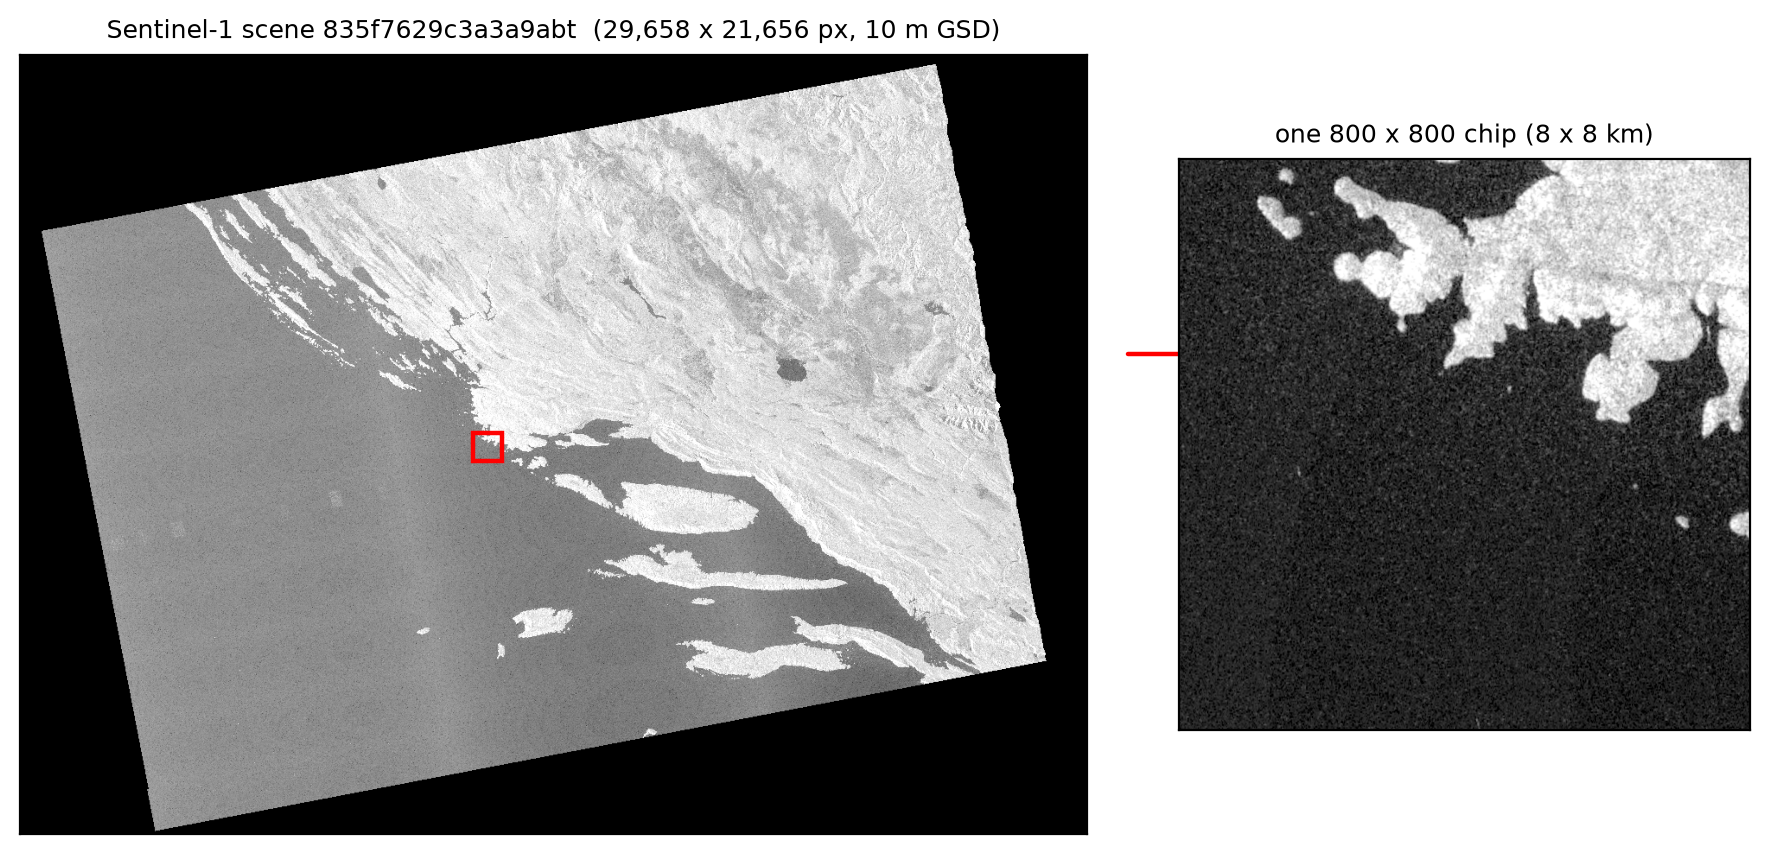
\includegraphics[width=\linewidth]{scene_context.png}\par
  \vspace{2mm}{\small One Sentinel-1 scene (about 300 $\times$ 220\,km) and
  one 800-pixel chip (8 $\times$ 8\,km).\par}
  \vspace{4mm}\raggedright
  \begin{itemize}
    \item 150 frozen study scenes: \textbf{111 train, 23 dev, 16 test}.
    \item Nested budgets: \textbf{12 $\subset$ 28 $\subset$ 56 $\subset$ 111}
      training scenes (10, 25, 50, 100\%).
    \item \textbf{50 near-shore, human-verified scenes}, opened once after
      test scoring: \PNFinalVessels{} vessels, \PNFinalDark{} dark,
      \PNFinalNearShore{} within 2\,km of shore.
    \item Input [VH, VV, VH − VV] in dB, 10\,m pixels.
  \end{itemize}
}
\calloutcolors
\block{Fix before the final cohort}{%
  BigEarthNet-S2 expects 10 optical bands. The first adapter kept 3 band
  kernels and scaled them by 10/3: first-layer weight norm
  \textbf{\PNStemWeightNormRatio}. A seeded 3-channel stem plus every other
  transferred tensor raised dev F1 from \PNStemDevBefore{} to
  \PNStemDevAfter{} (12 scenes). We then retrained \textbf{all
  \PNCells{} cells} from initialization.}
\normalcolors
% =====================================================================
\column{0.22}
\block{8 arms $\times$ 4 budgets = \PNCells{} cells}{
  \renewcommand{\arraystretch}{1.25}\setlength{\tabcolsep}{3mm}
  \begin{tabular}{@{}l>{\raggedright\arraybackslash}p{0.355\linewidth}>{\raggedright\arraybackslash}p{0.355\linewidth}@{}}
    \toprule
    Role & ViT-B/16 (86M) & ConvNeXt-V2-B (89M) \\
    \midrule
    \role{floor}{Random}     & fresh init       & fresh init \\
    \role{optical}{Optical}  & SatDINO (fMoW-RGB) & BigEarthNet-S2 \\
    \role{sar}{SAR}          & SARMAE (SAR-1M)  & BigEarthNet-S1 \\
    \role{imagenet}{ImageNet}& AugReg           & FCMAE \\
    \bottomrule
  \end{tabular}\par\vspace{5mm}
  Only the initialization changes inside a track. We compare domains
  \textbf{within} an architecture, then check whether the pattern repeats
  across the two.
}
\block{One shared point detector}{
  \centering
  % Poster-scale version of docs/class_report/figures/detector_pipeline.tex:
% two rows so it fits one 0.22 column at native type size.
\begin{tikzpicture}[font=\sffamily\normalsize, line width=1.8pt,
  >={Stealth[length=6mm, width=5mm]},
  stage/.style={draw, rounded corners=4pt, align=center, inner sep=8pt,
                minimum height=30mm, text=ink},
  data/.style={stage, fill=black!6, draw=black!45},
  enc/.style={stage, fill=rolesar!10, draw=rolesar!80!black, minimum width=66mm, minimum height=26mm},
  neck/.style={stage, fill=rolesar!5, draw=rolesar!60!black},
  cal/.style={stage, fill=roleoptical!15, draw=roleoptical!85!black},
  endst/.style={stage, fill=roleimagenet!12, draw=roleimagenet!80!black},
  flow/.style={->, draw=ink, rounded corners=3pt}]
\node[data, minimum width=50mm] (inp) {[VH, VV,\\ VH − VV]\\ 512² crop};
\node[enc, anchor=west] (vit) at ($(inp.east)+(18mm,13mm)$) {ViT-B/16, stride 16};
\node[enc, anchor=west] (cnn) at ($(inp.east)+(18mm,-13mm)$) {ConvNeXt-V2-B, s32 + up};
% tikzposter owns the pgf layer list, so the group box is drawn unfilled.
\node[draw=black!35, dashed, rounded corners=6pt, inner sep=5mm,
      fit=(vit)(cnn)] (encbox) {};
\node[anchor=south, font=\sffamily\small, text=black!60]
  at (encbox.north) {one encoder per track};
\node[neck, anchor=west, minimum width=40mm] (head) at ($(encbox.east)+(10mm,0)$) {shared\\ 256-ch\\ head};
\node[neck, anchor=north east, minimum width=62mm] (dec) at ($(head.south east)+(0,-16mm)$) {heatmap peaks\\ $\geq 0.05$, 120\,m NMS};
\node[cal, anchor=east, minimum width=60mm] (op) at ($(dec.west)+(-14mm,0)$) {threshold $\tau$\\ picked on dev};
\node[endst, anchor=east, minimum width=60mm] (mat) at ($(op.west)+(-14mm,0)$) {F1, 200\,m\\ geo match};
\draw[flow] (inp.east) -- ($(inp.east)+(8mm,0)$) |- (vit.west);
\draw[flow] (inp.east) -- ($(inp.east)+(8mm,0)$) |- (cnn.west);
\draw[flow] (encbox.east) -- (head.west);
\draw[flow] (head.south) -- (head.south |- dec.north);
\draw[flow] (dec) -- (op);
\draw[flow] (op) -- (mat);
\end{tikzpicture}
\par
  \vspace{5mm}\raggedright
  \begin{itemize}
    \item CenterNet-style Gaussian heatmap and focal loss; F1 with 200\,m
      geographic matching.
    \item Same optimizer, schedule, crops, data order and seed (0) for
      every cell. Strict FP32: \PNGpuHours{} H100 GPU-hours.
  \end{itemize}
}
\block{Once-only held-out protocol}{
  \centering
  % Once-only held-out protocol: each stage opens only after the previous one froze.
\begin{tikzpicture}[font=\sffamily\normalsize, line width=1.8pt,
  >={Stealth[length=6mm, width=5mm]},
  stage/.style={draw, rounded corners=4pt, align=left, inner sep=9pt,
               text width=0.74\linewidth, text=ink},
  num/.style={circle, fill=navy, text=white, font=\sffamily\bfseries\normalsize,
              minimum size=12mm, inner sep=0pt},
  flow/.style={->, draw=ink}]
\node[stage,fill=black!5, draw=black!40] (s1)
  {\textbf{Train \PNCells{} cells.} A sweep on 8 dev scenes picks each checkpoint and threshold.};
\node[stage,fill=rolesar!8, draw=rolesar!70!black, below=6mm of s1] (s2)
  {\textbf{Freeze the cohort.} Hash-bind every marker and checkpoint.};
\node[stage,fill=roleoptical!14, draw=roleoptical!85!black, below=6mm of s2] (s3)
  {\textbf{Score \PNTestScenes{} test scenes once.} Same thresholds, \textbf{no retuning}.};
\node[stage,fill=roleimagenet!12, draw=roleimagenet!80!black, below=6mm of s3] (s4)
  {\textbf{Open \PNFinalScenes{} verified scenes once.} Same thresholds, all \PNCells{} cells.};
\foreach \s/\n in {s1/1, s2/2, s3/3, s4/4} {
  \node[num, anchor=east] at ($(\s.west)+(-6mm,0)$) {\n};
}
\draw[flow] (s1) -- (s2);
\draw[flow] (s2) -- (s3);
\draw[flow] (s3) -- (s4);
\end{tikzpicture}
\par
}
% =====================================================================
\column{0.34}
\block{Pretraining helps most when labels are scarce}{
  \centering
  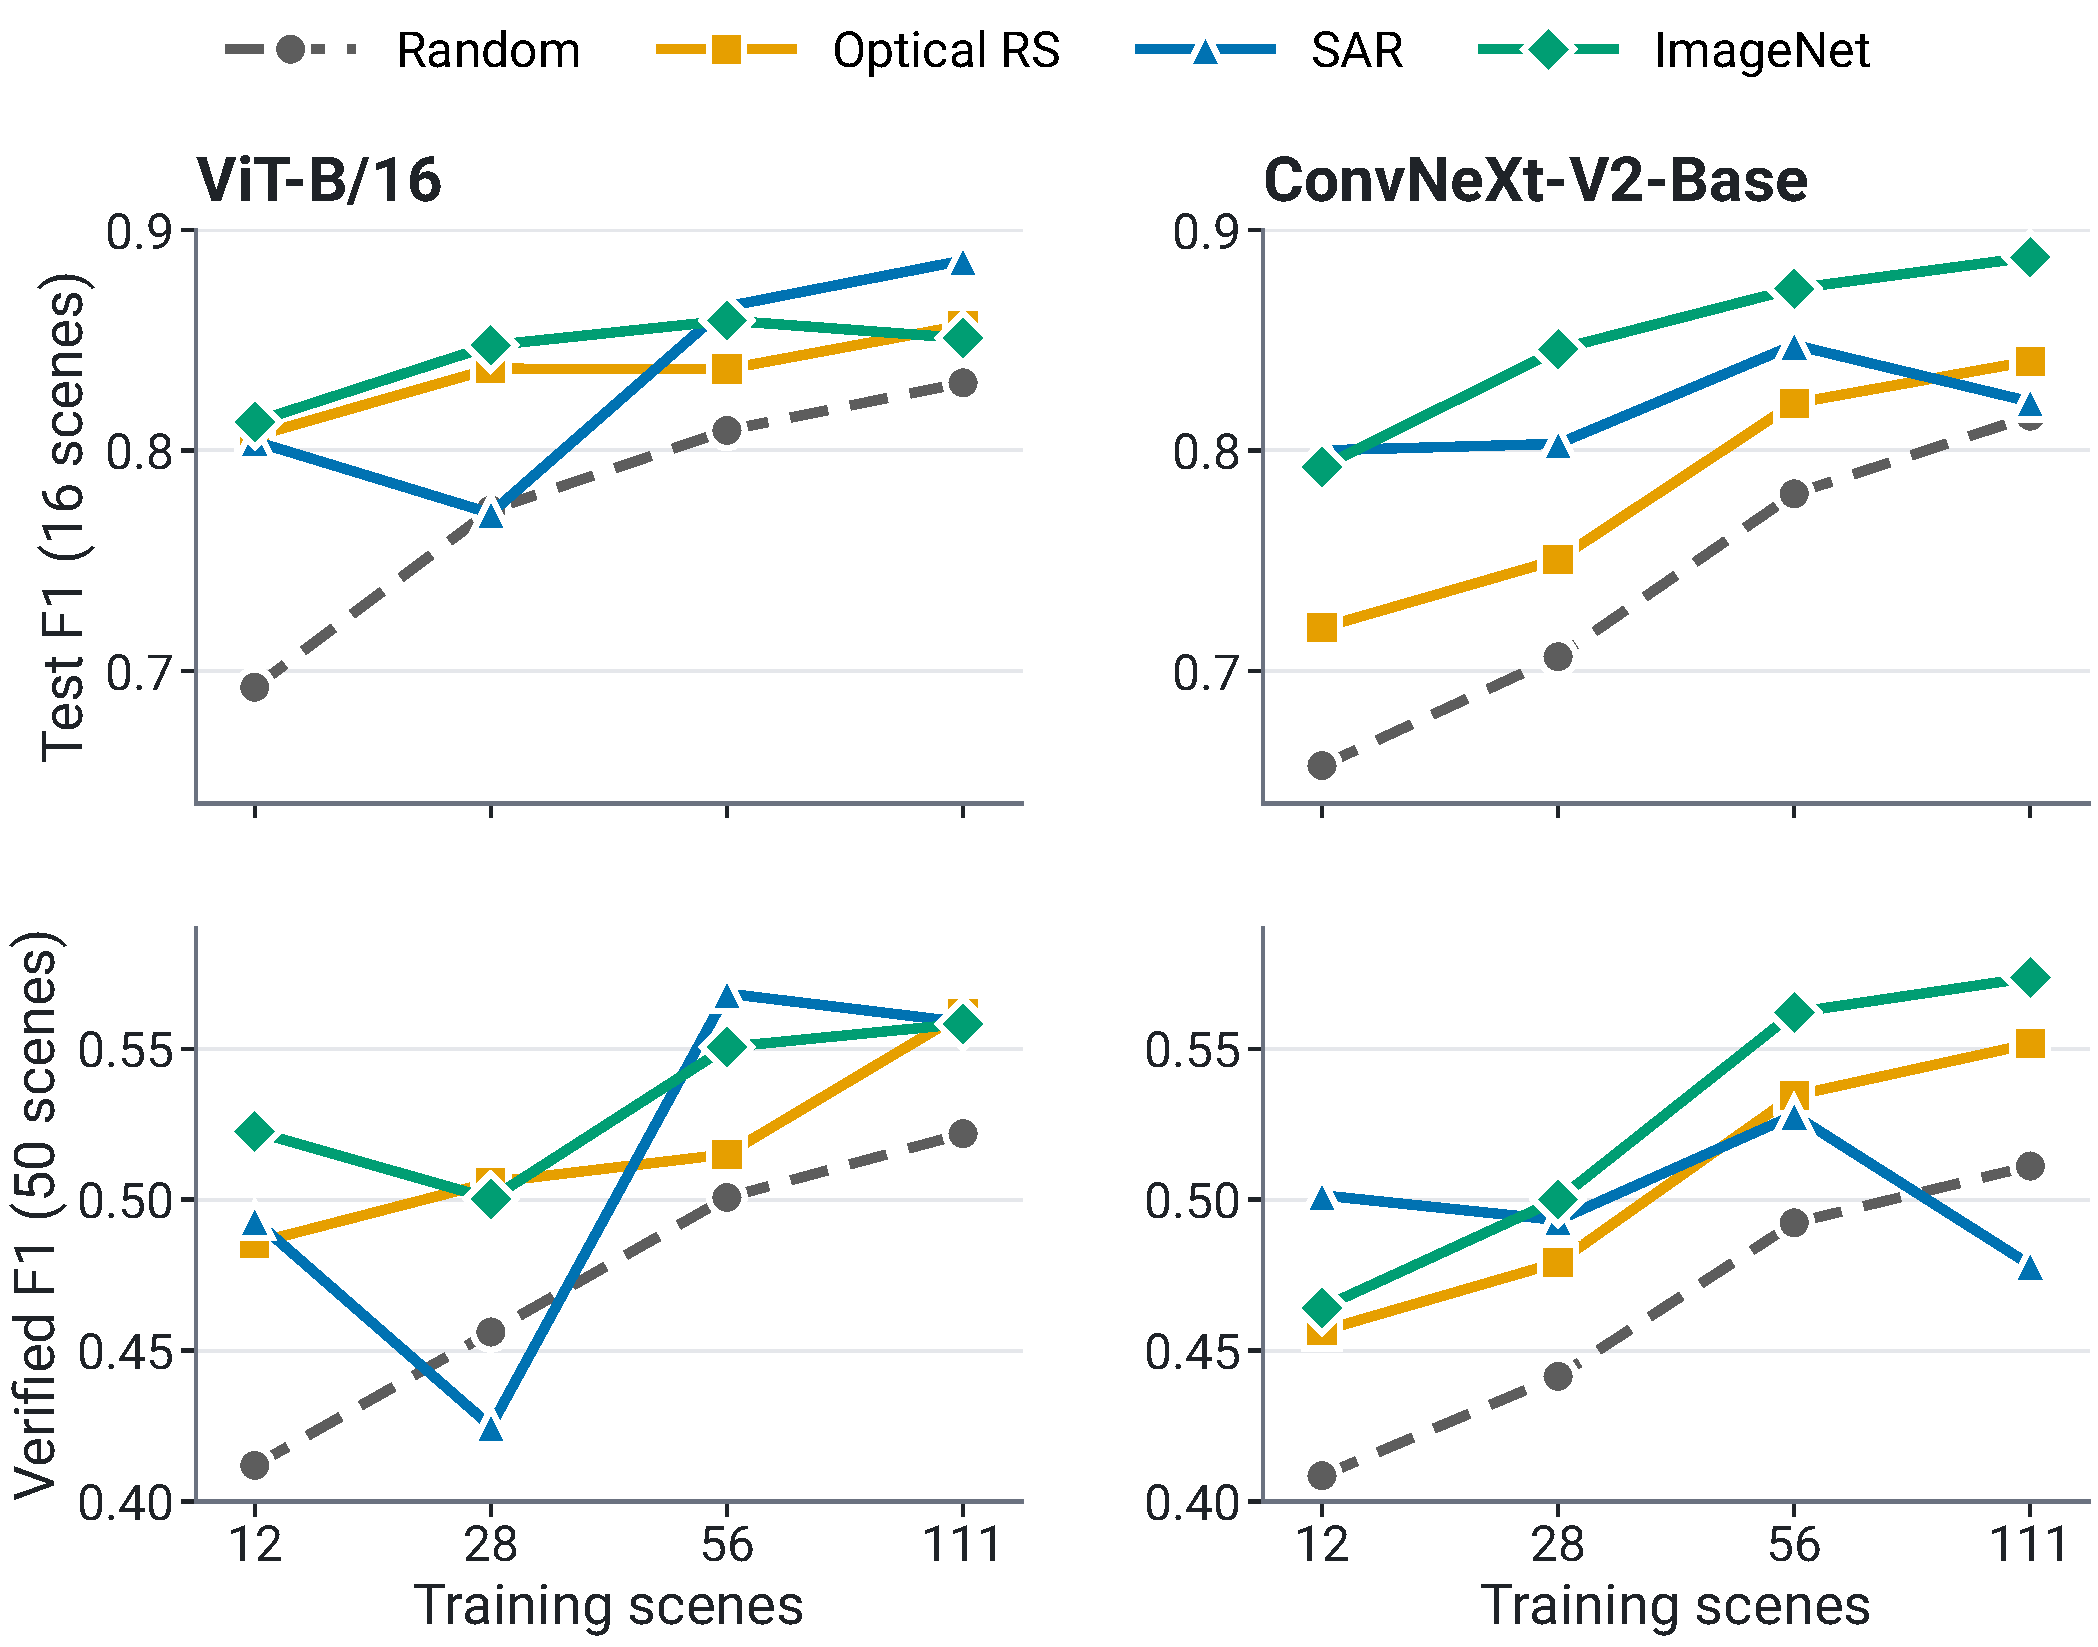
\includegraphics[width=\linewidth]{poster_label_efficiency.pdf}\par
  \vspace{5mm}\raggedright
  {\small F1 with 200\,m matching. Each of the \PNCells{} cells is scored once
  with the threshold it picked on 8 dev scenes. Top: \PNTestScenes{}
  held-out test scenes. Bottom: \PNFinalScenes{} near-shore, human-verified
  scenes. Seed 0; no intervals.\par}
}
\block{SAR vs.\ optical depends on backbone and budget}{
  \centering
  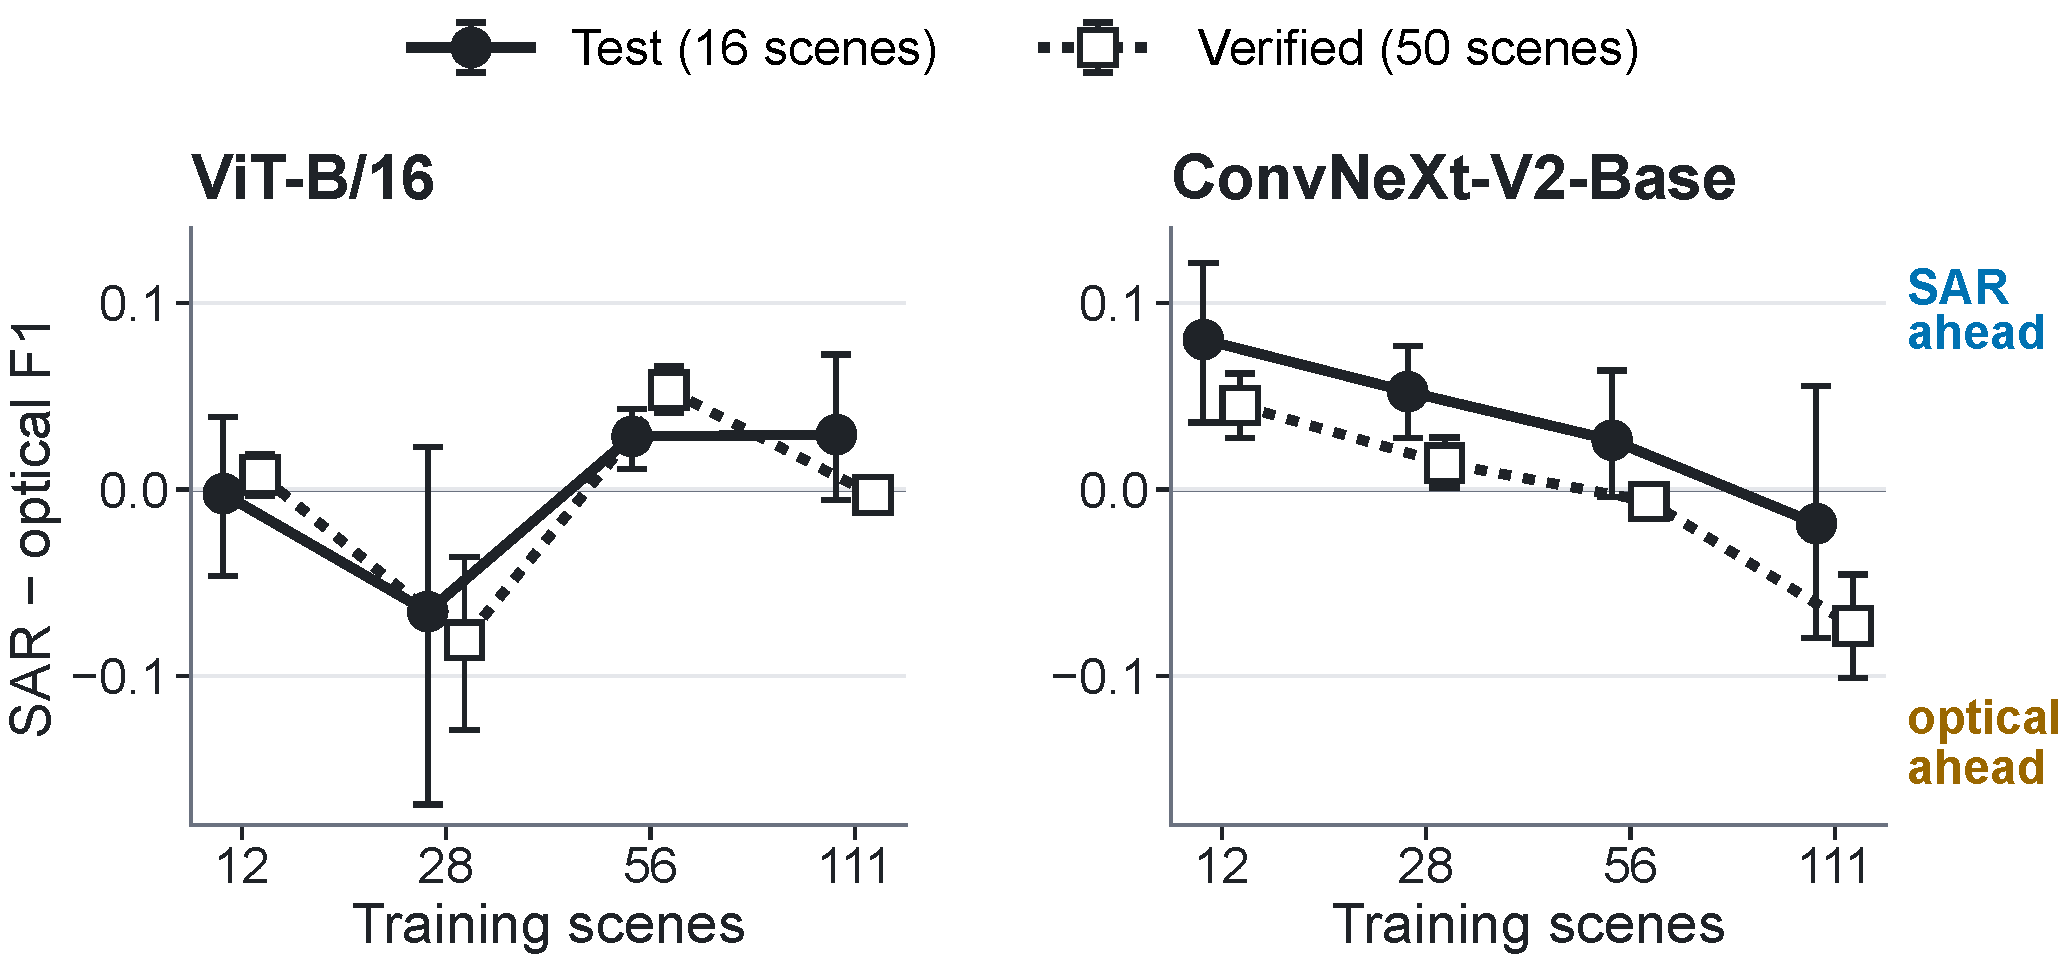
\includegraphics[width=\linewidth]{poster_sar_minus_optical.pdf}\par
  \vspace{5mm}\raggedright
  {\small Gray band: the largest test-F1 change across \PNRerunCells{} cells
  that we retrained with the same recipe and seed ($\pm$\PNRerunMax). A
  contrast inside the band is within rerun variation.\par}
}
\block{The verified scenes are a coastal stress test}{
  \centering
  \begin{tabular}{@{}c@{\hspace{14mm}}c@{\hspace{14mm}}c@{}}
    \statnum{\PNFinalFOneMin--\PNFinalFOneMax} &
    \statnum{$\le$\,\PNFinalDarkRecallMax} &
    \statnum{$\le$\,\PNFinalNearShoreFOneMax} \\[2mm]
    \statlabel{verified F1, all 32 cells\\(test: \PNTestFOneMin--\PNTestFOneMax)} &
    \statlabel{dark-vessel recall\\(\PNFinalDark{} dark vessels)} &
    \statlabel{near-shore F1\\(\PNFinalNearShore{} vessels within 2\,km)} \\
  \end{tabular}\par
  \vspace{5mm}\raggedright
  {\small Precision stays at \PNFinalPrecisionMin--\PNFinalPrecisionMax{}
  while recall falls to \PNFinalRecallMin--\PNFinalRecallMax: the
  detectors miss coastal vessels rather than over-fire.\par}
}
% =====================================================================
\column{0.22}
\block{Findings}{
  \begin{center}
    {\fontsize{64}{70}\selectfont\bfseries\color{roleimagenet}12 $\approx$ 111}\par
    \vspace{3mm}
    On the verified scenes, ImageNet ViT with 12 training scenes matches
    random ViT with 111 (\PNFinalVitBestTwelve{} vs.\
    \PNFinalVitRandomOneEleven{} F1).\par
  \end{center}
  \vspace{4mm}
  \begin{enumerate}
    \item \textbf{Pretraining pays off with few labels.} At 12 scenes every
      pretrained arm beats random: \PNTestGainTwelveMin{} to
      \PNTestGainTwelveMax{} test F1, \PNFinalGainTwelveMin{} to
      \PNFinalGainTwelveMax{} verified F1.
    \item \textbf{SAR beats optical only while labels are scarce.} CNN:
      \PNTestCnnSarMinusOptTen{} test F1 at 12 scenes,
      \PNTestCnnSarMinusOptHundred{} at 111. ViT: no stable order.
    \item \textbf{The input adapter matters.} With a seeded 3-channel stem,
      BigEarthNet-S2 beats random at every budget
      (\PNCnnOpticalTestGainMin{} to \PNCnnOpticalTestGainMax{} test F1).
    \item \textbf{Coastal and dark vessels stay hard.} Verified F1 is
      \PNFinalFOneMin--\PNFinalFOneMax{} (test: \PNTestFOneMin--\PNTestFOneMax).
      Dark-vessel recall $\le$ \PNFinalDarkRecallMax; near-shore
      F1 $\le$ \PNFinalNearShoreFOneMax.
  \end{enumerate}
}
\block{Limits}{
  \begin{itemize}
    \item One seed per cell; 8 dev scenes pick checkpoints and thresholds.
    \item The predeclared monotonicity gate failed: two SAR test curves
      drop by more than 0.02 as labels grow. We report the grid as
      descriptive.
    \item Checkpoints differ in objective and corpus as well as domain.
      We compare released checkpoints, not a causal domain effect.
  \end{itemize}
}
\block{Code and checkpoints}{
  \begin{tabular}{@{}c@{\hspace{12mm}}c@{}}
    \qrcode[height=7cm]{https://github.com/jroth1414/SAR-VesselBench} &
    \qrcode[height=7cm]{https://huggingface.co/roth1414/SAR-VesselBench} \\[3mm]
    \small GitHub: code, evidence & \small Hugging Face: weights
  \end{tabular}
}
\block{References}{
  \footnotesize\raggedright
  Paolo et al., xView3-SAR, NeurIPS 2022.
  Zhou et al., Objects as Points, 2019.
  Steiner et al., How to Train Your ViT?, TMLR 2022.
  Woo et al., ConvNeXt V2, CVPR 2023.
  Straka \& Gruber, SatDINO, 2025.
  Liu et al., SARMAE, CVPR 2026.
  Clasen et al., reBEN, IGARSS 2025.\par
}
\end{columns}
\end{document}
